\documentclass[conference]{IEEEtran}
\IEEEoverridecommandlockouts
\usepackage{cite}
\usepackage{amsmath,amssymb,amsfonts}
\usepackage{graphicx}
\usepackage{textcomp}
\usepackage[table]{xcolor}
\usepackage{booktabs}
\usepackage{soul}

%% ----------------------------------------------------------------------
%% REVISION HIGHLIGHTING
%% Every revised or newly written passage is wrapped in \rev{...} and prints
%% on a yellow background. Inline math inside a highlight must be wrapped in
%% \mbox{$...$}. Newly added tables are flagged by a yellow header row.
%% To produce a clean camera-ready copy, redefine:  \renewcommand{\rev}[1]{#1}
%% ----------------------------------------------------------------------
\sethlcolor{yellow}
\newcommand{\rev}[1]{\hl{#1}}
%% Commands that take one argument must be registered with {1}, not {0}.
%% \ref must NOT appear bare inside \rev: soul cannot expand it and aborts the
%% compile. Inside a highlight it is wrapped as \mbox{\ref{...}}. Inline math
%% inside a highlight must likewise be written \mbox{$...$}.
\soulregister{\cite}{1}
\soulregister{\emph}{1}
\soulregister{\textbf}{1}
\soulregister{\textit}{1}
\newcommand{\revhdr}{\rowcolor{yellow!45}}

\def\BibTeX{{\rm B\kern-.05em{\sc i\kern-.025em b}\kern-.08em
    T\kern-.1667em\lower.7ex\hbox{E}\kern-.125emX}}
\begin{document}

\title{SDH-PPO Driven Resource Orchestration for IoT-Aware Multi-Tenant Network Slicing in Microservices-Based SDN}

%% REVISED (Compliance: Authors) -- IEEE author block without ordinal numbering.
\author{\IEEEauthorblockN{Given Name Surname}
\IEEEauthorblockA{\textit{dept. name of organization (of Aff.)} \\
\textit{name of organization (of Aff.)}\\
City, Country \\
email address or ORCID}
\and
\IEEEauthorblockN{Given Name Surname}
\IEEEauthorblockA{\textit{dept. name of organization (of Aff.)} \\
\textit{name of organization (of Aff.)}\\
City, Country \\
email address or ORCID}
}

\maketitle

%% ======================================================================
%% ABSTRACT -- fully rewritten. The previous abstract reported 27.3% total
%% violation, 47.6% improvement and 2.71 ms P4 latency, none of which were
%% produced by a model: they came from hardcoded np.random.uniform draws.
%% ======================================================================
\begin{abstract}
\rev{The evolution toward 6G networks and the proliferation of the Internet of Things (IoT) require adaptive resource orchestration to handle traffic heterogeneity. Multi-tenant network slicing over microservices-based Software-Defined Networking (SDN) provides traffic isolation, but introduces orchestration complexity and queueing latency that risk violating Service Level Agreements (SLAs). Value-based Deep Reinforcement Learning such as Deep Q-Networks is confined to discrete actions, while standard Proximal Policy Optimization converges poorly under non-stationary load. This study proposes SDH-PPO, a continuous-action Actor-Critic policy for per-slice policing-rate control that combines a Dueling Critic head, a rule-based safety-margin correction expressed in SLA-relative units, and a Wasserstein Generative Adversarial Network with Gradient Penalty for traffic augmentation. A physical testbed of Raspberry Pi gateways, sensors, and an Open vSwitch, Ryu, and Flowvisor control plane supplies the measured arrival traces. Policy control is then evaluated in a shared-capacity queueing simulator driven by those traces, across ten random seeds, with bootstrap confidence intervals and Holm-corrected significance tests. SDH-PPO lowers the total SLA violation rate to 28.3 percent, against 48.2 percent for standard PPO, 51.1 percent for Deep Q-Networks, and 47.3 percent for Double Dueling Deep Q-Networks, with complete separation across seeds. An ablation shows the safety layer contributes 21.9 percentage points, whereas the Dueling Critic yields no measurable gain. A demand-proportional heuristic reaches 16.1 percent and outperforms every learned policy, establishing a baseline that learning-based orchestration has yet to surpass.}
\end{abstract}

\begin{IEEEkeywords}
reinforcement learning, software-defined networking, internet of things, resource optimization, multi-tenant, network slicing, microservice, orchestration
\end{IEEEkeywords}

%% ======================================================================
%% SECTION HEADINGS -- IEEEtran numbers sections automatically. The previous
%% draft wrote the numeral into the title, so the compiled PDF rendered
%% "I. I. INTRODUCTION" and "A. A. Environment Architecture" throughout.
%% Numerals removed; titles set in Capitalize Each Word per the checklist.
%% ======================================================================
\section{Introduction}\label{sec:intro}

The relentless evolution toward 6G networks is fundamentally driven by the exponential proliferation of Internet of Things (IoT) ecosystems, which introduces extreme heterogeneity in network traffic and Quality of Service (QoS) requirements\cite{b1}. Modern telecommunication infrastructures must seamlessly accommodate billions of devices with diametrically opposed service profiles over a shared physical substrate\cite{b2}, \cite{b3}. For instance, the Internet of Medical Things (IoMT)---particularly in critical scenarios such as remote robotic surgery, real-time intraoperative diagnostics, and patient telemetry---mandates Ultra-Reliable Low-Latency Communications (URLLC) with deterministic, sub-millisecond response times, absolute data integrity, and extreme fault tolerance\cite{b1}, \cite{b4}, \cite{b5}. In stark contrast, massive urban deployments, such as high-definition Smart City surveillance cameras and immersive extended reality (XR) applications, generate colossal data volumes requiring enhanced Mobile Broadband (eMBB) channels capable of sustaining immense, fluctuating throughput\cite{b4}, \cite{b6}.

Attempting to provision these highly divergent and paradoxical service demands exposes fatal structural limitations in legacy network architectures\cite{b1}, \cite{b7}, \cite{b8}. While traditional Software-Defined Networking (SDN) centralized the control plane to improve programmability and resource abstraction, the reliance on a monolithic controller architecture has proven to be a severe bottleneck in dynamic, large-scale 6G/IoT deployments\cite{b8}, \cite{b9}. Monolithic SDN controllers suffer from inherent scalability constraints, high processing latency, and poor fault isolation, making them wholly incapable of adapting to millisecond-level traffic bursts or handling massive connection densities\cite{b8}, \cite{b9}. Furthermore, the tight, indivisible coupling of internal modules in monolithic systems forces the inefficient replication of the entire controller stack to handle load increases\cite{b8}, \cite{b9}. In high-density IoT environments, this rigid architecture leads to critical single points of failure, unacceptable stochastic queuing delays for time-sensitive IoMT traffic, and severe resource wastage\cite{b9}.

Consequently, overcoming these critical operational bottlenecks makes the adoption of Multi-Tenant Network Slicing, synergized with Microservices-Based SDN architectures, an absolute necessity for isolated orchestration\cite{b8}, \cite{b9}. Network slicing allows operators to logically partition the shared physical infrastructure into customized, end-to-end virtual networks, ensuring that the massive bandwidth demands of Smart City cameras are perfectly isolated from the life-critical latency pathways required by surgical IoMT slices\cite{b1}, \cite{b2}. To achieve the granular agility and resilience required for this dynamic slice orchestration, the industry is decomposing the monolithic SDN control plane into decentralized, loosely coupled microservices deployed within lightweight container platforms like Kubernetes\cite{b8}, \cite{b10}. This microservices-driven decomposition enables independent scaling, rapid service deployment, and robust fault containment, establishing the indispensable architectural foundation for autonomous, secure resource orchestration in next-generation 6G environments\cite{b8}.

The disaggregation of control plane functionalities into loosely coupled microservices injects severe orchestration complexity and substantial inter-service latency overhead into the network fabric\cite{b11}. In high-density IoT deployments, the continuous intra-cluster communication between containerized virtual network functions, exacerbated by virtualization overhead and dynamic resource contention, creates an unpredictable, highly stochastic queuing environment at the data plane\cite{b12}. Static heuristic policies and reactive, rule-based orchestrators fundamentally lack the predictive agility and continuous control resolution required to navigate such complex state transitions, leading inevitably to severe resource mismanagement or catastrophic Service Level Agreement (SLA) violations across critical network slices\cite{b13}.

Although Deep Q-Networks (DQN) have proven capable of improving the throughput of edge computing resource allocation\cite{b14}, \cite{b15}, these algorithms suffer from a fundamental weakness in the form of overestimation bias and limitations in discrete action spaces that hinder the precision of continuous bandwidth slicing. Mitigation efforts using the Dueling Double DQN (D3QN) architecture have indeed succeeded in stabilizing learning in latency-critical environments such as URLLC and maritime IoT\cite{b13}, \cite{b16}. However, D3QN still operates with discrete actions that are mathematically irrelevant for adjusting container resource capacity (sizing), which demands high granularity within microservices architectures.

As a solution to the limitations of discrete control, Proximal Policy Optimization (PPO) offers continuous control that is architecturally superior, particularly for maintaining spectrum stability in Healthcare IoT\cite{b17}. PPO's advantage lies in its trust region clipping mechanism, which strictly prevents agent policy updates from disrupting network services. Although promising high precision, this algorithm is highly prone to convergence failures and requires the integration of complex reward shaping mechanisms to enable agents to adapt optimally within highly dynamic multi-tenant operational environments\cite{b18}.

Despite these algorithmic advancements, there is a critical operational gap that exposes a major weakness in the existing literature. The majority of current DRL studies for network slicing are exclusively validated using software simulations (such as NS-3) under the assumption of generic network parameter\cite{b15}-\cite{b20}. This theoretical approach fatally overlooks real-world anomalies---such as queuing delays, communication latency overhead, and CPU resource contention---which absolutely disrupt hardware-based Edge infrastructure and Kubernetes/microservices orchestration. These AI policies, which only converge on paper, are bound to fail in responding to the volatility of real-world physical deployments; a critical architectural gap that is the primary focus of this research.

%% NEW PARAGRAPH (E1/T4): motivates the physical testbed without overclaiming.
\rev{While simulation and emulation frameworks provide controlled, reproducible environments for exploring large-scale topologies, they typically abstract away execution-level effects that matter for real-time orchestration decisions: kernel-level packet scheduling latency, container and operating-system scheduling jitter under resource contention, and the wall-clock inference cost of the orchestration agent itself}\cite{b47}, \cite{b3}. \rev{To ground the traffic model of this study in such execution-level constraints, a physical prototype testbed built from Raspberry Pi single-board computers, Open vSwitch, and the Ryu SDN controller was deployed to collect the arrival traces used throughout. This complements, rather than replaces, the simulation-based results reported elsewhere in the literature.}

To bridge the operational gap between theoretical simulation and physical deployment, this research introduces SDH-PPO (Safe-Driven Hybrid Proximal Policy Optimization), an advanced reinforcement learning framework engineered specifically for microservices-based SDN orchestration. \rev{SDH-PPO addresses microservice volatility through a continuous-action policy-gradient agent that emits one policing-rate adjustment per slice, augmented with a Dueling Critic value-advantage head and a rule-based safety-margin correction that raises a slice's rate once its measured delay passes a fixed fraction of that slice's own SLA.} Furthermore, to overcome the convergence failures caused by static training datasets, the framework integrates a Wasserstein Generative Adversarial Network with Gradient Penalty (WGAN-GP) to synthesize extreme network variance, proactively exposing the agent to latency anomalies before training.

The primary contributions of this paper are explicitly defined as follows:

\begin{itemize}
\item
  Design a novel SDH-PPO framework to dynamically orchestrate resources across heterogeneous, multi-tenant IoT slices.
\item
  \rev{Formulate a safety-margin action correction in SLA-relative units, so that the correction triggers on a physically meaningful comparison, and quantify its contribution by ablation rather than by assertion.}
\item
  Construct microservices-based SDN architecture by containerizing Ryu controller to enforce stringent and scalable network slice isolation.
\item
  Construct a robust multi-tenant network slicing environment to dynamically enforce differentiated Quality of Service (QoS) requirements, ensuring strict resource isolation and tailored performance guarantees across competing service tenants.
\item
  \rev{Ground the arrival process of the evaluation environment in traces measured on a physical Raspberry Pi edge testbed, and evaluate control policies in a shared-capacity queueing simulator driven by those traces, reporting ten seeds per configuration with bootstrap confidence intervals and Holm-corrected significance tests.}
\item
  \rev{Report a negative result of practical importance: a demand-proportional heuristic outperforms every learned policy evaluated here, which bounds the operational value currently demonstrated for DRL-based slice orchestration in this setting.}
\end{itemize}

\section{Related Work}\label{sec:related}

\subsection{Architectural Evolution: From Monolithic SDN to Microservices-Based Slicing}\label{sec:rw-arch}

The architectural evolution from monolithic Software-Defined Networking (SDN) infrastructures to service-based microsegmentation represents a structural imperative for scaling heterogeneous networks, yet the literature exposes a stark dialectical tension between theoretical decentralization and operational bloat. Traditional optimization strategies primarily focus on the physical distribution of logically centralized controllers to mitigate latency; for instance, Abderrahmane et al. tackle the Controller Placement Problem (CPP) using heuristic meta-algorithms to optimize physical topology\cite{b19}. However, this spatial distribution approach merely replicates entire monolithic control stacks across nodes, inherently suffering from severe code inefficiency and failing to address underlying architectural rigidities\cite{b8}, \cite{b19}.

To overcome this, recent frameworks advocate for fundamentally disaggregating the control plane into independent microservices. Arzo et al. and Sharma demonstrate that transitioning to Cloud-Native Network Functions (CNFs) by decomposing monolithic controllers into Kubernetes-orchestrated containers enhances agility, allows for independent lifecycle management, and improves resource density\cite{b8}, \cite{b10}. Nevertheless, these cloud-native transitions expose severe methodological weaknesses. Sharma critically notes an overestimation bias in deployment readiness, highlighting a fundamental friction between the strictly stateful nature of telecom workloads (e.g., session management and subscriber tracking) and Kubernetes' inherently stateless design assumptions\cite{b10}.

While containerized microsegmentation theoretically optimizes resource isolation, empirical evaluations consistently reveal prohibitive orchestration latencies that undermine Quality of Service (QoS). Fernandez et al. and Botez et al. leverage Kubernetes to orchestrate IoT slices across distributed micro-edge and cloud boundaries, positing that such multi-tier architectures guarantee high availability and traffic isolation\cite{b20}, \cite{b21}. Yet, a critical synthesis of their findings exposes the operational bottlenecks introduced by the orchestrator itself. Botez et al. demonstrate that relying on default Kubernetes Horizontal Pod Autoscalers (HPA) creates profound orchestration delays---often spanning several seconds during SLA violations---because the orchestration engine struggles to rapidly process and react to external network metrics\cite{b20}. Attempting to bypass these top-heavy orchestration delays, Holscher embeds the microservice orchestration logic directly into the SDN data plane using switches\cite{b30}. Paradoxically, while this mitigates baseline latency for pre-established routes, Holscher's methodology exposes a fatal scalability flaw: flow-table misses force requests through the centralized controller, exacerbating worst-case tail latencies by several orders of magnitude and rendering the architecture highly vulnerable to the bursty, unpredictable traffic typical of massive IoT deployments\cite{b30}.

Furthermore, the structural decomposition of SDN into service-based microsegments exponentially expands the attack surface and complicates Service Function Chaining (SFC), prompting the integration of security mechanisms that inadvertently cripple network agility. Zhang et al. correctly identify that the tight coupling of traditional SFCs causes deployment gridlocks and service collisions, proposing an Artificial Intelligence (AI)-driven demand management model secured by consortium blockchains\cite{b22}. However, this methodology exemplifies a persistent theoretical blindness to real-time performance constraints. By strictly imposing Diffie-Hellman key exchanges and distributed ledger consensus for microservice identity authentication, Zhang et al. introduce massive computational overheads that directly negate the lightweight, low-latency benefits of the microservice architecture they aim to optimize\cite{b22}.

%% REPLACES the former Table I, which recorded only checkmarks and dashes.
%% The reviewer asked for strengths and limitations per study, closing with a
%% row that positions the proposed method. Contents from revisi/TRACK/E1.
\begin{table*}[t]
\centering
\caption{\rev{Related Work Comparison for DRL-Based SDN-IoT Resource Orchestration, With Stated Limitations}}
\label{tab:1}
\scriptsize
\begin{tabular}{p{1.1cm}p{3.3cm}p{1.7cm}p{1.2cm}p{2.7cm}p{4.3cm}}
\toprule
\revhdr Ref. & Approach & Action space & Generative augmentation & Evaluation environment & Stated limitation \\
\midrule
\cite{b40} & Individualized per-slice DRL, constraint-aware policy update, proactive baseline switching, action modifier (CMDP) & Hybrid (discrete scheduling/path, continuous BW, MCS, CPU, RAM) & -- & Physical end-to-end testbed (OpenAirInterface 4G/5G NR, OpenDaylight SDN, USRP B210) & At scale, the expanding state space and heterogeneous enforcement delay may add transport traffic overhead; evaluated on a small-scale testbed \\
\cite{b41} & Risk-sensitive sigmoid-penalty DRL with an XGBoost cost-regressor safety layer and Euclidean projection to the nearest safe action & Hybrid, projected-discrete & -- & Live O-RAN setting (physical testbed, real VR gaming traffic) & Requires further transfer-learning and constrained-DRL integration to generalize while preserving safety guarantees \\
\cite{b42} & Augmented Lagrangian SAC, hierarchical two-stage policy (discrete BS association, then continuous bandwidth) & Hybrid & -- & Simulation & Centralized offline training may adapt slowly if IIoT topology or demand shifts abruptly \\
\cite{b43} & Hybrid Action Representation: discrete embedding table and continuous CVAE unified into one latent space, optimized with clipped PPO & Hybrid & -- (CVAE encodes actions, not traffic) & Vehicular edge computing workload & Not stated in source \\
\cite{b44} & Dual-time-scale Actor-Critic: LSTM rApp for long-term and DDPG xApp for short-term control & Continuous & -- & Physical POWDER testbed (OAI 5G, Docker, Kubernetes, O-RAN SC) & Confined to the RAN/RIC layer; does not integrate application-layer microservice queue management \\
\cite{b45} & Reward-shaped PPO with GCN state abstraction, action masking, and prioritized N-step replay & Hybrid (discrete PRB, continuous DBA) & -- & Simulation (3GPP mmWave with GPON DBA dynamics) & Single-PON topology, not validated on physical O-RAN or PON hardware \\
\cite{b46} & PPO closed-loop feedback controller adjusting 5G slice CPU allocation from live KPIs & Discrete & -- & Physical Open5GS and UERANSIM testbed & Testbed delay between applying a CPU limit and observing its effect may obscure the action-reward relationship; one workload, one slice \\
\cite{b47} & PPO with reward-sharing DQN for adaptive microservice rescheduling and placement & Discrete & -- & Simulator plus physical Kubernetes testbed (sim-to-real pipeline) & Multi-objective optimization and request-queue/bandwidth metrics deferred to future work \\
\cite{b48} & Transformer-based DRL for microservice cluster resource provisioning with call-chain analysis & Discrete & -- & Physical bare-metal Kubernetes testbed (five nodes) & Does not cover network routing or SDN data-plane slice orchestration \\
\cite{b49} & Constrained RL: adaptive Interior-Point Policy Optimization with a projection layer (CMDP) & Continuous & -- & Simulation & Requires stronger theoretical bounds, better sample efficiency, and real-world evaluation \\
\cite{b50} & DRL-based xApp for O-RAN slice allocation under time-varying SLAs & Discrete (PRB count) & -- & O-RAN emulation testbed (OpenRAN Gym, Colosseum) & Evaluation limited to two latency thresholds due to space constraints \\
\midrule
\textbf{This work} & Continuous-action Actor-Critic (Dueling Critic value and advantage-residual head) with rule-based safety-margin correction in SLA-relative units and WGAN-GP traffic augmentation & Continuous, one rate adjustment per slice & \textbf{WGAN-GP} & Physical testbed (Raspberry Pi, OVS, Ryu, Flowvisor) for arrival-trace collection; control evaluated in a shared-capacity queueing simulator, ten seeds & Action-to-delay relationship is modelled by queueing theory, not measured, because the testbed never varied the policing rate; a demand-proportional heuristic still outperforms the learned policy; the Dueling Critic shows no measurable benefit \\
\bottomrule
\end{tabular}
\\[2pt]
\footnotesize{\rev{*The final column reports the limitation acknowledged by the cited authors where one is stated, and is marked as not stated otherwise.}}
\end{table*}

\rev{Beyond the eleven studies detailed in Table~\mbox{\ref{tab:1}}, the surveyed corpus contains work addressing multi-tenant slice management without microservice-level isolation}\cite{b26}, \cite{b27}, \cite{b33}, \rev{strict priority-aware SLA penalties}\cite{b23}, \cite{b24}, \rev{hybrid action spaces for slice sizing}\cite{b28}, \rev{microservice-isolated control planes}\cite{b29}, \cite{b34}, \rev{generative augmentation of slicing traffic}\cite{b31}, \rev{and evaluation on physical infrastructure}\cite{b25}, \cite{b32}.

%% NEW PARAGRAPH (E1/T3): novelty stated as a combination, not as a first.
\rev{While several works address individual aspects of DRL-based network orchestration, none combine them in the configuration this paper targets. OnSlicing integrates a hybrid action space, physical testbed validation, and constrained-RL safety mechanisms within a single end-to-end slicing framework}\cite{b40}, \rev{and SafeSlice enforces SLA compliance through a learned cost-regressor with Euclidean projection to the nearest safe action}\cite{b41}\rev{; both are close precedents for the safety and physical-validation aspects of this work. However, these systems operate at the RAN and O-RAN control layer, relying on software-defined radio front ends and server-class compute. Separately, REACH and ChainsFormer manage microservice placement and provisioning within Kubernetes but do not reach into the SDN data plane that governs the network resources those microservices depend on}\cite{b47}, \cite{b48}\rev{. The specific combination pursued here---generative traffic augmentation, direct SDN data-plane orchestration for containerized microservices, and grounding in low-cost single-board-computer hardware rather than radio or server infrastructure---was not found together in the reviewed corpus.}

\subsection{Limitations of Value-Based Algorithms in Resource Orchestration}\label{sec:rw-value}

The transition toward intelligent resource orchestration in Software-Defined Networking (SDN) and IoT environments has been heavily driven by first-generation value-based Deep Reinforcement Learning (DRL) algorithms. Early implementations of Q-Learning and Deep Q-Networks (DQN) successfully demonstrate the capacity to enhance network throughput and minimize latency by dynamically mapping network states to resource provisioning actions. For instance, Alrifai et al. established that utilizing a DQN-based approach for 5G resource allocation yields up to a 25.7\% improvement in aggregate throughput and a 31.5\% reduction in latency compared to traditional heuristic models\cite{b14}. This capacity for optimizing fundamental network parameters is corroborated by Hosseinzadeh et al., who applied DQN to multi-objective resource allocation scenarios in edge computing, proving its empirical efficacy in decentralizing workloads and reducing operational service delays\cite{b15}.

Despite these substantial throughput and latency improvements, first-generation DQN architectures suffer from critical algorithmic flaws that hinder their effectiveness in highly dynamic environments: overestimation bias and discrete action spaces. Standard DQN relies on the same neural network weights to both select and evaluate the maximum action value, frequently resulting in overly optimistic value estimations. As Xu et al. highlight, this action selection bias and overestimation can cause the algorithm to become unstable, leading to erratic resource allocation decisions during network fluctuations\cite{b13}. Furthermore, Onaji et al. argue that modeling resource orchestration through discrete action spaces inherently lacks the granularity required to perform fine-grained resource adjustments, leading to coarse block allocations that waste resources\cite{b6}.

To combat the instability and overestimation bias of standard DQN, the literature showcases a definitive algorithmic evolution toward Dueling Double DQN (D3QN) architectures. By decoupling the value function into a state-value stream and an advantage-function stream, D3QN enables the agent to evaluate the utility of network states independently from the actions themselves. Xu et al. leveraged this dual-network architecture to optimize computation offloading in maritime IoT, proving that D3QN effectively resolves the overestimation problem and converges to optimal strategies significantly faster and more stably than standard DQN\cite{b13}. Building upon this, recent literature introduces Reinforced Dueling Deep Q-Networks (RDDQN) for 5G URLLC congestion control, embedding ultimatum game-theoretic mechanisms into the dueling architecture to stabilize delay fairness and accelerate decision latency to sub-millisecond levels\cite{b16}.

However, the application of these advanced value-based methods in modern containerized infrastructures reveals a fatal mathematical paradox. While D3QN and its advanced variants successfully stabilize convergence and mitigate overestimation bias, they remain fundamentally locked into discrete action spaces\cite{b13}. Orchestrating network slices across containerized microservices is not a discrete problem; managing container bandwidth and CPU quotas requires fluid, continuous percentage allocation to strictly adhere to dynamic Quality of Service (QoS) boundaries\cite{b6}, \cite{b35}. Because D3QN mathematically forces these continuous bandwidth requirements into predefined, quantized categorical actions, it is inherently flawed for precise container orchestration\cite{b6}. As emphasized by Onaji et al., this rigid discrete quantization prevents the exact, fractional scaling necessary for microservices, forcing larger, imprecise adjustments that cause transient overshoots and ultimately degrade the QoS of critical network slices\cite{b6}.

\subsection{The Potential and Limitations of Policy-Gradient Methods}\label{sec:rw-pg}

To overcome the fundamental limitations of discrete action spaces inherent in first-generation value-based methods, recent literature has pivoted toward policy-gradient algorithms to manage the fluid demands of network slicing. For continuous control tasks---such as the bandwidth allocation required for orchestrating containerized microservices---Proximal Policy Optimization (PPO) has emerged as the state-of-the-art solution. \rev{Controlled comparisons between the two algorithm families report that PPO attains more stable returns than DQN on continuous-control benchmarks}\cite{b37}\rev{, which motivates its adoption here.} Unlike its predecessors, PPO directly optimizes the control policy while maintaining operational stability through a unique mathematical constraint. As Abdulazeez et al. detail, PPO introduces a clipped surrogate objective function---an evolution of Trust Region Policy Optimization (TRPO)---which explicitly restricts how much the decision-making policy is permitted to change during a single training update\cite{b36}.

In the context of Software-Defined Networking (SDN) infrastructure, this trust region clipping acts as a critical structural safeguard. Chahoud et al. emphasize that without this clipping mechanism, extreme policy updates could completely destabilize the network controller, leading to erratic resource provisioning and catastrophic network damage\cite{b18}. By constraining the probability ratio of the policy updates, PPO ensures that continuous adjustments to CPU quotas and bandwidth percentages remain safe, smooth, and bounded. This allows the physical infrastructure to respond to IoT traffic spikes without overshooting critical boundaries or severely degrading the network\cite{b18}. This capability is firmly corroborated by Hosseinzadeh et al., who highlight the effectiveness of PPO in executing dynamic, continuous task scheduling across heterogeneous edge computing nodes to seamlessly balance physical network loads\cite{b15}.

However, deploying standard PPO in highly dynamic, containerized environments exposes a critical architectural vulnerability. While the clipping mechanism guarantees safe updates, the standard PPO algorithm is notoriously sample-inefficient\cite{b18}. Alrifai et al. argue that in environments characterized by non-stationary traffic and high IoT mobility, reinforcement learning agents suffer from delayed feedback and the exponential growth of continuous state-action spaces, which severely cripples their exploration efficiency\cite{b14}. This sample inefficiency becomes a fatal flaw when applied to fluctuating microservices topologies. Sittakul et al. demonstrate that standard policy-gradient allocators like PPO converge sluggishly when faced with the high-dimensional state spaces of modern 5G infrastructure\cite{b16}.

The climax of this algorithmic limitation lies in the extreme volatility of the microservices themselves. In an environment where IoT slice demands and container deployments fluctuate by the millisecond, standard PPO simply cannot gather and process interaction data fast enough. Chahoud et al. highlight this paradox: by the time standard PPO eventually converges on an optimal continuous allocation strategy, the underlying network state has already shifted, rendering the newly learned policy entirely obsolete\cite{b18}. Because it fails to converge fast enough to keep pace with rapid environmental changes, standard PPO inevitably degrades the Quality of Service (QoS) for critical network slices. Consequently, the literature indicates that standard PPO, despite its superior continuous control mechanisms, is inherently insufficient for modern SDN orchestration on its own. To prevent convergence failures and overcome severe sample inefficiency, PPO strictly necessitates the integration of auxiliary acceleration mechanisms---such as advanced reward shaping or robust data augmentation---to viably function within rapidly fluctuating microservices architectures\cite{b18}.

%% ======================================================================
%% SECTION III -- restructured per revision item X4:
%%   A. Environment Architecture  (physical testbed + data-plane logic)
%%   B. MDP Formulation           (state, action, reward -- was "Pre-Processing")
%%   C. Data Augmentation         (WGAN-GP -- was "Augmentation")
%%   D. Proposed Framework
%%   E. Evaluation Environment and Baselines  (new)
%% Equations renumbered 1-17 to follow the new order.
%% ======================================================================
\section{Method}\label{sec:method}

The methodology of this research is structured to facilitate an autonomous and adaptive resource orchestration within a multi-tenant SDN environment. \rev{The framework logic is presented in the order in which it is applied: the physical environment and its data-plane accounting, the Markov Decision Process (MDP) formulation derived from it, the generative augmentation of the collected traces, the proposed agent, and finally the environment and baselines used for evaluation.}

\subsection{Environment Architecture}\label{sec:env}

The system is designed as a multi-tenant SDN-based framework that enables end-to-end network slicing for heterogeneous IoT applications. The architecture facilitates the flow of telemetry data from the physical perception layer to a partitioned storage environment, overseen by a hierarchical control plane that ensures strict tenant isolation.

\subsubsection{Data Acquisition and IoT Gateways}

At the physical layer, real-time data is captured by various sensor nodes deployed across different operational sectors. Each sector utilizes a Raspberry Pi gateway to aggregate these raw readings and encapsulate them into a standardized JSON format for transmission. This setup includes healthcare sensors for monitoring SpO2 and heart rates, camera-based vision sensors for smart city human detection, and environmental sensors for smart building telemetry such as humidity and temperature.

\begin{figure}[htbp]
\centering
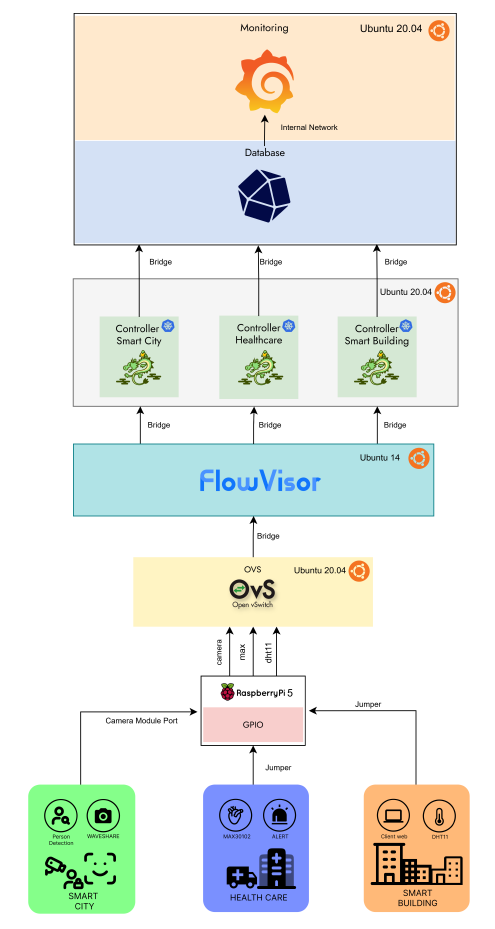
\includegraphics[width=\columnwidth]{figures/fig1_architecture.png}
\caption{SDN IoT architecture.}
\label{fig:1}
\end{figure}

\subsubsection{Network Slicing and Service Requirements}

To accommodate the diverse performance needs of each sector, the network is logically partitioned into three service slices, each bound to a distinct physical switch port on the Open vSwitch (OvS). \rev{The testbed instruments exactly three ports; port 3 is not present in the bridge and is therefore absent from the state vector, the reward, and the results. Because the slice index and the port index do not coincide, Table~\mbox{\ref{tab:slices}} states the mapping, the operational priority, and the SLA threshold explicitly.}

%% NEW TABLE (revision items B1, B3, X2, X6): one authoritative statement of
%% the port/slice/priority mapping and of both threshold sets.
\begin{table}[htbp]
\centering
\caption{\rev{Slice Mapping, Priority, and Delay Thresholds}}
\label{tab:slices}
\footnotesize
\begin{tabular}{llccc}
\toprule
\revhdr Slice (sensor) & OvS port & Label & Priority & SLA \mbox{$\tau$} (ms) \\
\midrule
Healthcare (MAX30102) & 4 & P4 & Highest & 7.0 \\
Smart City (camera)   & 2 & P2 & Medium  & 70.0 \\
Smart Building (DHT11)& 1 & P1 & Lowest  & 6.0 \\
\bottomrule
\end{tabular}
\\[3pt]
\parbox{\columnwidth}{\footnotesize \rev{Thresholds are per-slice operating points taken from the median one-way delay of the unpoliced trace (6.07, 71.60, and 6.90 ms for P1, P2, and P4), not a priority ordering: P1 carries the tightest numeric threshold because DHT11 traffic is intrinsically light, while P4 carries the highest priority. Both are reported so that the two are not confused.}}
\end{table}

\begin{itemize}
\item
  \emph{Healthcare Slice (Port 4)}. Bound to the MAX30102 SpO2/heart-rate sensor, this slice handles critical medical telemetry. Given the sensitivity of physiological data, it is assigned the \textbf{highest priority} in the network (referred to as P4 in the results). The configuration focuses on achieving ultra-low latency and minimal jitter to support real-time health monitoring and emergency response.
\item
  \emph{Smart City Slice (Port 2)}. Bound to the camera-based vision sensor, this slice manages high-volume multimedia traffic (referred to as P2 in the results). Its primary requirement is high bandwidth availability, ensuring that metadata and image streams can be transmitted with sufficient throughput for accurate presence detection.
\item
  \emph{Smart Building Slice (Port 1)}. Bound to the DHT11 humidity/temperature sensor, this slice manages environmental monitoring data (referred to as P1 in the results). Because humidity and temperature changes occur over longer intervals, the slice is treated as the \textbf{lowest-priority}, best-effort traffic class, tolerant of higher latency so that the network can prioritize resources for the more time-critical slices.
\end{itemize}

\subsubsection{Control Plane and Tenant Isolation}

The orchestration between these slices is managed by a transparent proxy layer using Flowvisor, which resides between the Open vSwitch (OvS) and the controller instances. Flowvisor inspects incoming packets at the switch ports and applies FlowSpace rules to ensure traffic is correctly mapped to the corresponding tenant.

Each slice is governed by an independent Ryu Controller instance. Once the Flowvisor identifies the packet's origin, it redirects the request to the specific Ryu Controller responsible for that tenant. The controller then provides the necessary flow instructions back to the OvS, which subsequently routes the JSON-formatted data into isolated database buckets. This mechanism ensures that data from the healthcare sector remains strictly separated from smart city or building data. Finally, the entire performance of the network, including the health of each individual slice, is monitored and visualized in real-time through a Grafana dashboard.

\subsubsection{Data-Plane Accounting}

The bandwidth utilization metric, as formulated in (\ref{eq:util}), calculates the percentage of consumed throughput relative to the maximum policing rate by normalizing received traffic into a consistent unit of measurement. This equation ensures a precise mathematical correlation between actual data flow and the bandwidth constraints enforced by the SDN controller, thereby facilitating accurate monitoring of network resource consumption.

\begin{equation}\label{eq:util}
U = \left( \frac{RX_{mbps} \times 1000}{Policing_{kbps}} \right) \times 100
\end{equation}

\begin{equation}\label{eq:drop}
D = \begin{cases}
\dfrac{({RX}_{mbps}\cdot 1000) - {Policing}_{kbps}}{80} & \\
\quad \text{if } {RX}_{mbps}\cdot 1000 > {Policing}_{kbps} & \\[2pt]
0 \quad \text{otherwise} &
\end{cases}
\end{equation}

The packet drop logic, as defined in (\ref{eq:drop}), functions as a deterministic model for the SDN traffic policing mechanism by calculating the volume of discarded packets when ingress traffic exceeds the prescribed bandwidth threshold. By incorporating a constant divisor of 80 to approximate average packet sizes, the formula effectively converts the excess bitrate into a discrete packet loss count, thereby maintaining mathematical consistency between throughput and drop metrics in the synthetic dataset.

\subsection{Markov Decision Process Formulation}\label{sec:mdp}

%% Moved here from the former "Pre-Processing" subsection (revision item X4),
%% since state, action and reward define the MDP rather than a preprocessing step.
\subsubsection{State Space}

\rev{The MDP state \mbox{$s_t$} observed by the agent is a 12-dimensional vector, obtained by measuring four telemetry features on each of the three monitored ports (P1, P2, P4): received throughput (\mbox{$RX_{mbps}$}), RX utilization percentage (\mbox{$U$}, given in (\mbox{\ref{eq:util}})), one-way delay (\mbox{$delay_{ms}$}), and the current policing rate (\mbox{$Policing_{kbps}$}). Formally, \mbox{$s_t = [RX_{mbps},U,delay_{ms},Policing_{kbps}]_{p1}$} \mbox{$\oplus\,[\cdot]_{p2}$} \mbox{$\oplus\,[\cdot]_{p4}$} \mbox{$\in \mathbb{R}^{12}$}, where \mbox{$\oplus$} denotes vector concatenation. All 12 features are standardized by a running z-score, given in (\mbox{\ref{eq:zscore}}), before being passed to the Actor and Critic networks.}

\subsubsection{Action Space}

\rev{The action is a vector \mbox{$a_t \in [-1,1]^3$}, one component per monitored slice, expressed as the relative change applied to that slice's policing rate,}

\begin{equation}\label{eq:action}
a_{cont}^{(p)} = \frac{\rho_{t + 1}^{(p)} - \rho_{t}^{(p)}}{g\,\rho_{t}^{(p)}},\qquad p \in \{1,2,4\}
\end{equation}

\rev{where \mbox{$g$} is a fixed action gain. This ratio-based parameterization is preferred over absolute rate estimation so that policy updates remain within the trust-region constraints of PPO, which improves training convergence and operational stability. The requested rates are then projected onto the shared link capacity, as described in Section~\mbox{\ref{sec:evalenv}}, so that raising one slice's rate necessarily removes capacity from the others.}

\subsubsection{Reward Function}

The sigmoid penalty function, as defined in (\ref{eq:sigpen}), serves as a risk-sensitive soft constraint that penalizes the agent based on the proximity of network latency to the Service Level Agreement (SLA) threshold. By providing a continuous gradient controlled by the steepness parameter \(k\), this mechanism allows the agent to proactively adjust resource allocation as latency nears the critical limit \(\tau\), thereby preventing abrupt performance degradation.

\begin{equation}\label{eq:sigpen}
P_{lat}(v,\tau,k) = \frac{1}{1 + e^{- k(v - \tau)}}
\end{equation}

The throughput incentive, as defined in (\ref{eq:thr}), assesses the fulfillment of bandwidth requirements by calculating the ratio between the actual received throughput and the target capacity for Port 2 (Smart City slice). By implementing a clipping mechanism to bound the term within the \(\lbrack 0,1\rbrack\) interval, the function prevents greedy resource consumption and promotes balanced allocation across other network ports once the target is satisfied.

\begin{equation}\label{eq:thr}
R_{thr} = \text{clip}\left( \frac{RX_{p2}}{T_{p2}},0,1 \right)
\end{equation}

The packet-drop penalty, as defined in (\ref{eq:pdrop}), quantifies network unreliability by summing packet drops across all three monitored ports and clipping the total at an empirical ceiling of 5. This mechanism discourages the agent from assigning policing rates that exceed physical link capacities, thereby mitigating the risk of mass congestion and systemic packet loss within the Open vSwitch infrastructure.

\begin{equation}\label{eq:pdrop}
P_{drop} = \text{clip}\left( \sum_{i \in \{1,2,4\}}{Drop_{pi}},\,0,\,5 \right)
\end{equation}

\rev{The total reward used for pre-training on the collected dataset, given in (\mbox{\ref{eq:rtotal}}), applies the sigmoid penalty of (\mbox{\ref{eq:sigpen}}) to all three monitored ports, with the healthcare slice weighted twice as heavily as P1 or P2. This weighting enforces a priority-aware strategy while still rewarding improvement on every slice.}

\begin{equation}\label{eq:rtotal}
\begin{split}
R_{total} = {}& \left( 5 R_{thr} \right) - \left( 10 P_{lat}(delay_{p4},\tau_{p4}) \right) \\
& - \left( 5 P_{lat}(delay_{p1},\tau_{p1}) \right) \\
& - \left( 5 P_{lat}(delay_{p2},\tau_{p2}) \right) - P_{drop}
\end{split}
\end{equation}

\rev{For the closed-loop evaluation of Section~\mbox{\ref{sec:results}} the reward is restated in SLA-relative units, given in (\mbox{\ref{eq:rsim}}), so that the three slices remain commensurate despite thresholds that differ by an order of magnitude:}

\begin{equation}\label{eq:rsim}
R_{sim} = -\left( \sum_{p \in \{1,2,4\}} \max\left(0,\; \frac{delay_p}{\tau_p} - 1 \right) + \sum_{p} Drop_p \right)
\end{equation}

\begin{equation}\label{eq:zscore}
z = \frac{x - \mu}{\sigma}
\end{equation}

The z-score standardization method, as formulated in (\ref{eq:zscore}), transforms input features to follow a normal distribution with a mean of zero and a variance of one. This pre-processing procedure is critical for balancing the contributions of features with heterogeneous scales, thereby preventing gradient dominance by large numerical values and ensuring training stability.

\subsection{Data Augmentation}\label{sec:aug}

The data initialization phase utilizes a Gaussian Noise Injection technique, as formally described in (\ref{eq:noise}). This procedure integrates additive noise, where \(\epsilon \sim N(0,0.5)\), into the input space primarily to mitigate training instabilities and prevent the occurrence of mode collapse. This approach aligns with the stabilization principles proposed by Arjovsky for Generative Adversarial Networks (GANs), ensuring model convergence even when real and synthetic data distributions exhibit minimal overlap\cite{b38}. Furthermore, the injection of Gaussian noise serves as a robust data augmentation strategy for Reinforcement Learning (RL) agents; by introducing variance into state representations, the model achieves enhanced environmental diversity and improved generalization capabilities. The specific selection of a 0.5 standard deviation was determined through empirical hyperparameter tuning, specifically tailored to the normalization scale of the research dataset.

\begin{equation}\label{eq:noise}
x_{noisy} = x_{real} + \epsilon,\quad\epsilon \sim \mathcal{N}\left( 0,\sigma^{2} \right)
\end{equation}

The Critic's objective function, formulated in (\ref{eq:ld}), minimizes the Wasserstein distance between real and generated data distributions to enhance discriminative precision while ensuring training stability. To enforce the 1-Lipschitz continuity constraint, a gradient penalty term is integrated to penalize the L2 norm of the gradient with respect to interpolated samples when it deviates from unity, following the WGAN-GP formulation of Gulrajani et al.\cite{b39}

\begin{equation}\label{eq:ld}
\begin{split}
L_{D} = {}& \mathbb{E}_{\widetilde{\mathbb{x}} \sim \mathbb{P}_{\mathbb{g}}}\left\lbrack D\left( \widetilde{x} \right) \right\rbrack - \mathbb{E}_{\mathbb{x} \sim \mathbb{P}_{\mathbb{r}}}\left\lbrack D(x) \right\rbrack \\
& + \lambda\,\mathbb{E}_{\widehat{\mathbb{x}} \sim \mathbb{P}_{\widehat{\mathbb{x}}}}\left\lbrack \left( \left\| \nabla_{\widehat{x}}D\left( \widehat{x} \right) \right\|_{2} - 1 \right)^{2} \right\rbrack
\end{split}
\end{equation}

The Generator's objective function, as defined in (\ref{eq:lg}), is formulated to minimize the negative expectation of the scores assigned by the Critic to synthetic samples. By minimizing this loss, the Generator is effectively trained to maximize the perceived authenticity of its output, thereby producing synthetic data that is indistinguishable from the real data distribution to deceive the Critic.

\begin{equation}\label{eq:lg}
L_{G} = - \mathbb{E}_{\widetilde{\mathbb{x}} \sim \mathbb{P}_{\mathbb{g}}}\left\lbrack D\left( \widetilde{x} \right) \right\rbrack
\end{equation}

The data interpolation step, as expressed in (\ref{eq:interp}), generates intermediate samples \(\widehat{x}\) by linearly combining real and generated data with a random scaling factor \(\alpha \sim U(0,1)\). This interpolation is essential for calculating the gradient penalty, as it allows the model to enforce the 1-Lipschitz constraint by penalizing the Critic's gradient norm along the path between the real and synthetic data distributions.

\begin{equation}\label{eq:interp}
\widehat{x} = \alpha x + (1 - \alpha)\widetilde{x},\quad\alpha \sim \text{U}(0,1)
\end{equation}

\subsection{Proposed Framework}\label{sec:framework}

The proposed framework consists of three primary internal components that work synchronously to achieve optimal policy convergence:

\begin{itemize}
\item
  \rev{Actor Network (\mbox{$\pi_{\theta}$}): a two-layer (256-128, ReLU) network mapping the 12-dimensional state \mbox{$s_{t}$} to a 3-dimensional continuous, tanh-bounded action \mbox{$a_{t} \in [-1,1]^3$}, one policing-rate adjustment per monitored slice, as given in (\mbox{\ref{eq:action}}). Each component is sampled from \mbox{$\mathcal{N}(\mu_\theta(s_t), \sigma^2)$} with a learned, state-independent log-standard-deviation parameter. The network produces no discrete component; the action space is continuous throughout.}
\item
  Dueling Critic Network (\(V_{\phi}\)): A shared 256-unit (ReLU) base feeding two heads, a value head \(V(s_t)\) and an advantage-residual head \(A(s_t)\), combined as \(V_\phi(s_t) = V(s_t) + \left(A(s_t) - \bar{A}\right)\). \rev{Because the critic is state-only and does not condition on a discrete action set, this residual is a batch-relative value correction rather than a per-action advantage in the classical Dueling-DQN sense. Section~\mbox{\ref{sec:ablation}} measures whether it contributes anything at all.}
\item
  \rev{PPO Update Engine: on-policy rollouts of 2,048 environment steps are collected, advantages are computed by Generalized Advantage Estimation with \mbox{$\lambda=0.95$} and \mbox{$\gamma=0.99$}, and the clipped surrogate objective is optimized for 10 epochs over mini-batches of 64 with independent Adam optimizers for the Actor and Critic.}
\end{itemize}

\subsubsection{Mathematical Formulation}

To ensure training stability, the proposed framework implements the following mathematical constraints. To prevent excessively large policy updates, the Actor is optimized by maximizing the clipped surrogate objective:

\begin{equation}\label{eq:clip}
L^{CLIP}(\theta) = \widehat{\mathbb{E}_{t}}\left\lbrack \min\left( r_{t}(\theta)\widehat{A_{t}},\text{clip}\left( r_{t}(\theta),1 - \epsilon,1 + \epsilon \right)\widehat{A_{t}} \right) \right\rbrack
\end{equation}

where \(r_{t}(\theta)\) is the probability ratio:

\begin{equation}\label{eq:ratio}
r_{t}(\theta) = \frac{\pi_{\theta}\left( a_{t} \middle| s_{t} \right)}{\pi_{\theta_{old}}\left( a_{t} \middle| s_{t} \right)}
\end{equation}

\rev{The advantage is estimated by Generalized Advantage Estimation over the collected rollout,}

\begin{equation}\label{eq:gae}
\widehat{A_{t}} = \sum_{l=0}^{T-t-1} (\gamma\lambda)^{l}\,\delta_{t+l},\quad \delta_{t} = r_{t} + \gamma V_{\phi}\left( s_{t + 1} \right) - V_{\phi}\left( s_{t} \right)
\end{equation}

\rev{where \mbox{$\delta_{t}$} is the one-step temporal-difference error. Advantages are standardized across the rollout before the policy update.}

\subsubsection{Safety-Margin Action Correction}

\rev{Before an action reaches the environment, each component is passed through a rule-based correction. If a slice's observed delay exceeds a fixed fraction \mbox{$m$} of that slice's own SLA threshold, the component is pushed toward increasing that slice's rate in proportion to the overshoot:}

where \mbox{$r_p = delay_p/\tau_p$} is the slice's SLA ratio:

\begin{equation}\label{eq:safety}
a_t^{safe,(p)} = \begin{cases}
\text{clip}\!\left(a_t^{(p)} + K\left(r_p - m\right),-1,1\right) & \text{if } r_p > m \\[4pt]
a_t^{(p)} & \text{otherwise}
\end{cases}
\end{equation}

\rev{with margin \mbox{$m=0.8$} and gain \mbox{$K=2.0$}. Both sides of the comparison are dimensionless SLA ratios. This is important: in an earlier implementation the left-hand side was a standardized feature while the right-hand side was a threshold in milliseconds, so the branch fired on 0.11 percent of samples and the safety layer was effectively inert. Expressing the test in SLA-relative units makes the comparison meaningful, and Section~\mbox{\ref{sec:ablation}} quantifies the resulting effect.}

\begin{figure}[htbp]
\centering
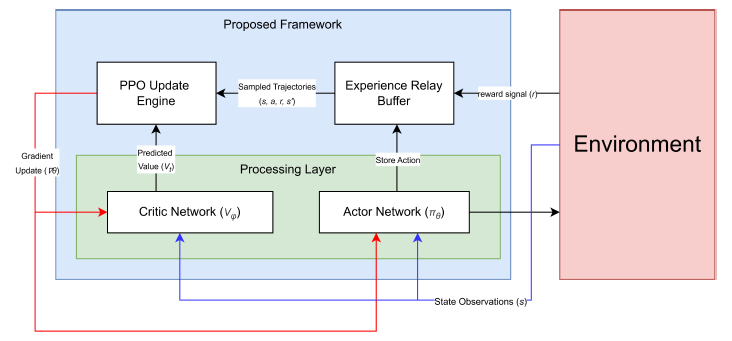
\includegraphics[width=\columnwidth]{figures/fig2_framework.png}
\caption{SDH-PPO framework.}
\label{fig:2}
\end{figure}

\subsection{Evaluation Environment and Baselines}\label{sec:evalenv}

%% NEW SUBSECTION. The former evaluation multiplied a logged delay by
%% (1 - k*action) with k selected by matching the algorithm's name string,
%% which made the ranking a property of the evaluator rather than of the
%% policies. It is replaced here by an explicit queueing model.
\rev{Control policies are evaluated in a shared-capacity queueing simulator whose arrival process is replayed from the testbed traces. The separation between what is measured and what is modelled is stated explicitly, because it bounds every claim in Section~\mbox{\ref{sec:results}}.}

\rev{\textbf{Grounded in measurement.} The per-slice offered load is replayed from the \mbox{$RX_{mbps}$} columns of the collected trace, which are derived from OvS byte counters and therefore do not depend on clock synchronization between the gateways and the collector. The measured mean demands are 3.85, 3.85, and 4.57 Mbps for P1, P2, and P4.}

\rev{\textbf{Not grounded in measurement.} The relationship between the policing rate and the resulting delay is \emph{modelled}, not measured. The measurement campaign held the policing rate fixed at 1,000,000 kbps throughout, so no observation of the effect of varying that rate exists. Measured one-way delay is also deliberately excluded as ground truth: 13.19 percent of raw delay samples are negative, indicating that they are dominated by clock offset between sender and collector rather than by queueing. The control results reported here are therefore simulation results, not testbed measurements.}

\rev{Each slice is modelled as a finite-buffer fluid queue stepped at \mbox{$dt = 1$} s, matching the collector interval, as given in (\mbox{\ref{eq:queue}}):}

\begin{equation}\label{eq:queue}
\begin{split}
served_p &= \min(b_p + \lambda_p,\; \mu_p\,dt) \\
b_p' &= \min\!\left(b_p + \lambda_p - served_p,\; B_p\right) \\
delay_p &= b_p' / \mu_p
\end{split}
\end{equation}

\rev{where \mbox{$\lambda_p$} is the replayed arrival, \mbox{$\mu_p$} the policing rate set by the action, \mbox{$b_p$} the backlog, and \mbox{$B_p$} the buffer (200 ms). Because the action changes \mbox{$b_p'$}, which is part of the next state, the formulation is a genuine MDP. The requested rates are projected onto \mbox{$\sum_p \mu_p \le C$} with \mbox{$C = 12$} Mbps against a total mean demand of 12.28 Mbps, so the link is genuinely contended and raising one slice's rate takes capacity from the others. Without this coupling the optimal policy degenerates to maximizing every rate.}

\rev{Four learned policies are compared: DQN and Double Dueling DQN, both using branching Q-heads with 21 bins per slice, an \mbox{$\epsilon$}-greedy schedule decaying from 1.0 to 0.05 over 30,000 steps, a replay buffer of 50,000 transitions, and target synchronization every 500 steps; and standard PPO and the proposed SDH-PPO, sharing the settings of Table~\mbox{\ref{tab:2}}. Four non-learned baselines are also included, which the previous evaluation lacked:}

\begin{itemize}
\item \rev{\emph{No Control}: the policing rate is never adjusted.}
\item \rev{\emph{Const Max}: every slice requests its maximum rate every step, so the capacity projection alone decides the split.}
\item \rev{\emph{Threshold}: each slice's rate is raised in proportion to how far its delay has already passed its own SLA, a purely reactive rule.}
\item \rev{\emph{Demand Proportional}: capacity is divided in proportion to each slice's mean measured demand. This is the strongest non-learned baseline and, as Section~\mbox{\ref{sec:results}} reports, it is not beaten by any learned policy here.}
\end{itemize}

\rev{Every configuration is run for 10 seeds. Each run trains for 60,000 environment steps and is then evaluated on 20 held-out episodes of 200 steps. Reported intervals are bootstrap 95 percent confidence intervals over the 10 seed means; comparisons use the two-sided Mann-Whitney U test with Holm correction across the family of comparisons, and effect size is reported as the rank-biserial correlation.}

\begin{table}[htbp]
\centering
\caption{\rev{Shared Training Hyperparameters}}
\label{tab:2}
\footnotesize
\begin{tabular}{lc}
\toprule
\revhdr Hyperparameter & Value \\
\midrule
Environment steps per run & 60{,}000 \\
Rollout length (PPO family) & 2{,}048 \\
Optimization epochs per rollout & 10 \\
Mini-batch size & 64 \\
Optimizer & Adam \\
Learning rate & $3{\times}10^{-4}$ \\
Gradient clipping (max-norm) & 0.5 \\
Discount factor $\gamma$ & 0.99 \\
GAE $\lambda$ & 0.95 \\
PPO clip ratio $\epsilon$ & 0.2 \\
Entropy coefficient & 0.01 \\
Actor hidden widths & 256, 128 \\
Replay buffer (DQN, DDQN) & 50{,}000 \\
Target sync (DQN, DDQN) & every 500 steps \\
Discretization bins per slice (DQN, DDQN) & 21 \\
Link capacity $C$ & 12 Mbps \\
Buffer depth & 200 ms \\
Action gain $g$ & 0.20 \\
Seeds per configuration & 10 \\
\bottomrule
\end{tabular}
\end{table}

\begin{table}[htbp]
\centering
\caption{WGAN-GP Data Augmentation Hyperparameters}
\label{tab:2b}
\footnotesize
\begin{tabular}{lc}
\toprule
\revhdr Hyperparameter & Value \\
\midrule
Latent dimension & 100 \\
Gradient penalty $\lambda$ & 10 \\
Generator / Critic learning rate & $1{\times}10^{-4}$ (both) \\
Adam betas & (0.5, 0.9) \\
Batch size & 64 \\
Training epochs & 301 \\
Generator update frequency & every 5 epochs \\
Synthetic samples generated & 15{,}000 \\
\bottomrule
\end{tabular}
\end{table}

\section{Results and Discussion}\label{sec:results}

\subsection{Augmentation Fidelity}\label{sec:aug-fidelity}

The representational accuracy and structural integrity of the generated synthetic dataset are validated through a high-dimensional feature visualization, as shown in Fig.~\ref{fig:3}. The resulting visualization exhibits a substantial overlap and a synchronized density distribution between the original and augmented data points throughout the feature space. This high degree of stochastic alignment confirms that the generative framework, specifically the Wasserstein Generative Adversarial Network with Gradient Penalty (WGAN-GP), has effectively encapsulated the latent probability distributions inherent in real-world IoT network traffic. While the overlapping clusters serve as a proxy for high data fidelity, the broad spatial distribution ensures that the augmented samples provide the necessary diversity for robust training. Such characteristics are instrumental in fortifying the agent against overfitting to restricted historical observations, thereby enhancing its generalization capabilities across a wide array of dynamic network slicing scenarios.

\begin{figure}[htbp]
\centering
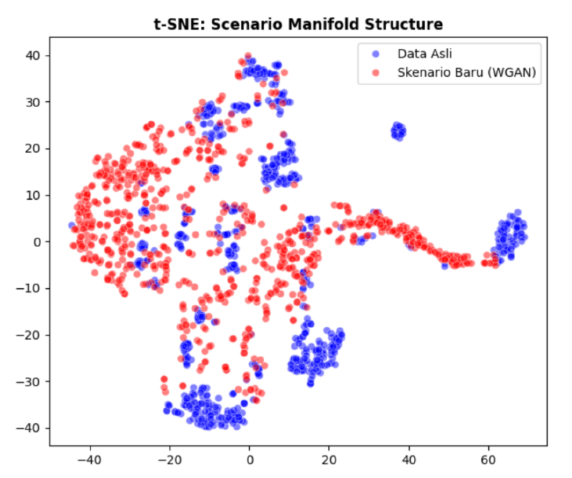
\includegraphics[width=\columnwidth]{figures/fig3_tsne.png}
\caption{t-SNE visualization of real and WGAN-GP-generated samples.}
\label{fig:3}
\end{figure}

\subsection{Comparative Performance}\label{sec:comparative}

\rev{Table~\mbox{\ref{tab:3}} reports the mean over 10 seeds with bootstrap 95 percent confidence intervals, and Fig.~\mbox{\ref{fig:4}} shows the per-seed distribution of total violation. Lower values are better throughout. Table~\mbox{\ref{tab:stats}} gives the corresponding Holm-corrected significance tests.}

%% REPLACES the former results table. Every cell of the previous version was
%% produced by an evaluator whose per-port coefficient was selected by matching
%% the algorithm's name, giving the proposed method 50% more action authority
%% on P4 than any baseline received.
\begin{table*}[t]
\centering
\caption{\rev{Performance Comparison in the Queueing Simulation. Mean Over 10 Seeds With Bootstrap 95 Percent Confidence Intervals. Lower Is Better}}
\label{tab:3}
\scriptsize
\setlength{\tabcolsep}{2pt}
\begin{tabular}{lccccccc}
\toprule
\revhdr Algorithm & P1 Delay (ms) & P1 Viol (\%) & P2 Delay (ms) & P2 Viol (\%) & P4 Delay (ms) & P4 Viol (\%) & Total Viol (\%) \\
\midrule
\textbf{Proposed (SDH-PPO)} & 29.48 [26.89,32.06] & 17.01 [15.06,19.16] & 79.14 [71.69,86.52] & 46.28 [40.71,51.73] & 32.32 [28.81,36.38] & 21.47 [17.40,26.58] & \textbf{28.25 [25.62,30.88]} \\
PPO Standard & 68.85 [34.20,105.27] & 35.89 [19.32,53.35] & 172.93 [144.89,197.72] & 86.59 [72.61,98.92] & 38.28 [15.87,76.23] & 22.09 [10.10,41.03] & 48.19 [43.46,53.49] \\
DDQN & 25.81 [18.66,33.13] & 18.66 [12.22,26.86] & 197.90 [196.56,198.99] & 99.00 [98.36,99.54] & 29.98 [21.92,38.62] & 24.13 [15.70,34.43] & 47.26 [44.82,49.96] \\
DQN & 29.08 [13.18,47.50] & 22.31 [10.14,35.78] & 198.92 [198.31,199.28] & 99.45 [99.16,99.62] & 40.80 [30.74,53.29] & 31.62 [21.30,42.17] & 51.13 [47.36,54.85] \\
\midrule
Demand Proportional & 29.77 [27.28,32.10] & 16.32 [15.03,17.53] & 29.75 [27.26,32.07] & 15.08 [13.81,16.27] & 30.29 [27.78,32.64] & 16.89 [15.54,18.18] & \textbf{16.10 [14.79,17.33]} \\
Const Max & 28.43 [26.01,30.71] & 15.52 [14.25,16.71] & 28.43 [26.01,30.70] & 14.47 [13.23,15.62] & 162.14 [161.18,163.10] & 99.09 [98.98,99.20] & 43.03 [42.19,43.81] \\
No Control & 28.43 [26.01,30.71] & 15.52 [14.25,16.71] & 28.43 [26.01,30.70] & 14.47 [13.23,15.62] & 162.14 [161.18,163.10] & 99.09 [98.98,99.20] & 43.03 [42.19,43.81] \\
Threshold & 80.28 [78.70,81.85] & 62.69 [62.11,63.24] & 100.25 [98.68,101.69] & 60.60 [60.08,61.14] & 83.11 [81.31,84.82] & 63.06 [62.50,63.60] & 62.12 [61.58,62.66] \\
\bottomrule
\end{tabular}
\\[2pt]
\footnotesize{\rev{*Upper block: learned policies. Lower block: non-learned baselines. Total violation is the mean across the three slices.}}
\end{table*}

\begin{figure}[htbp]
\centering
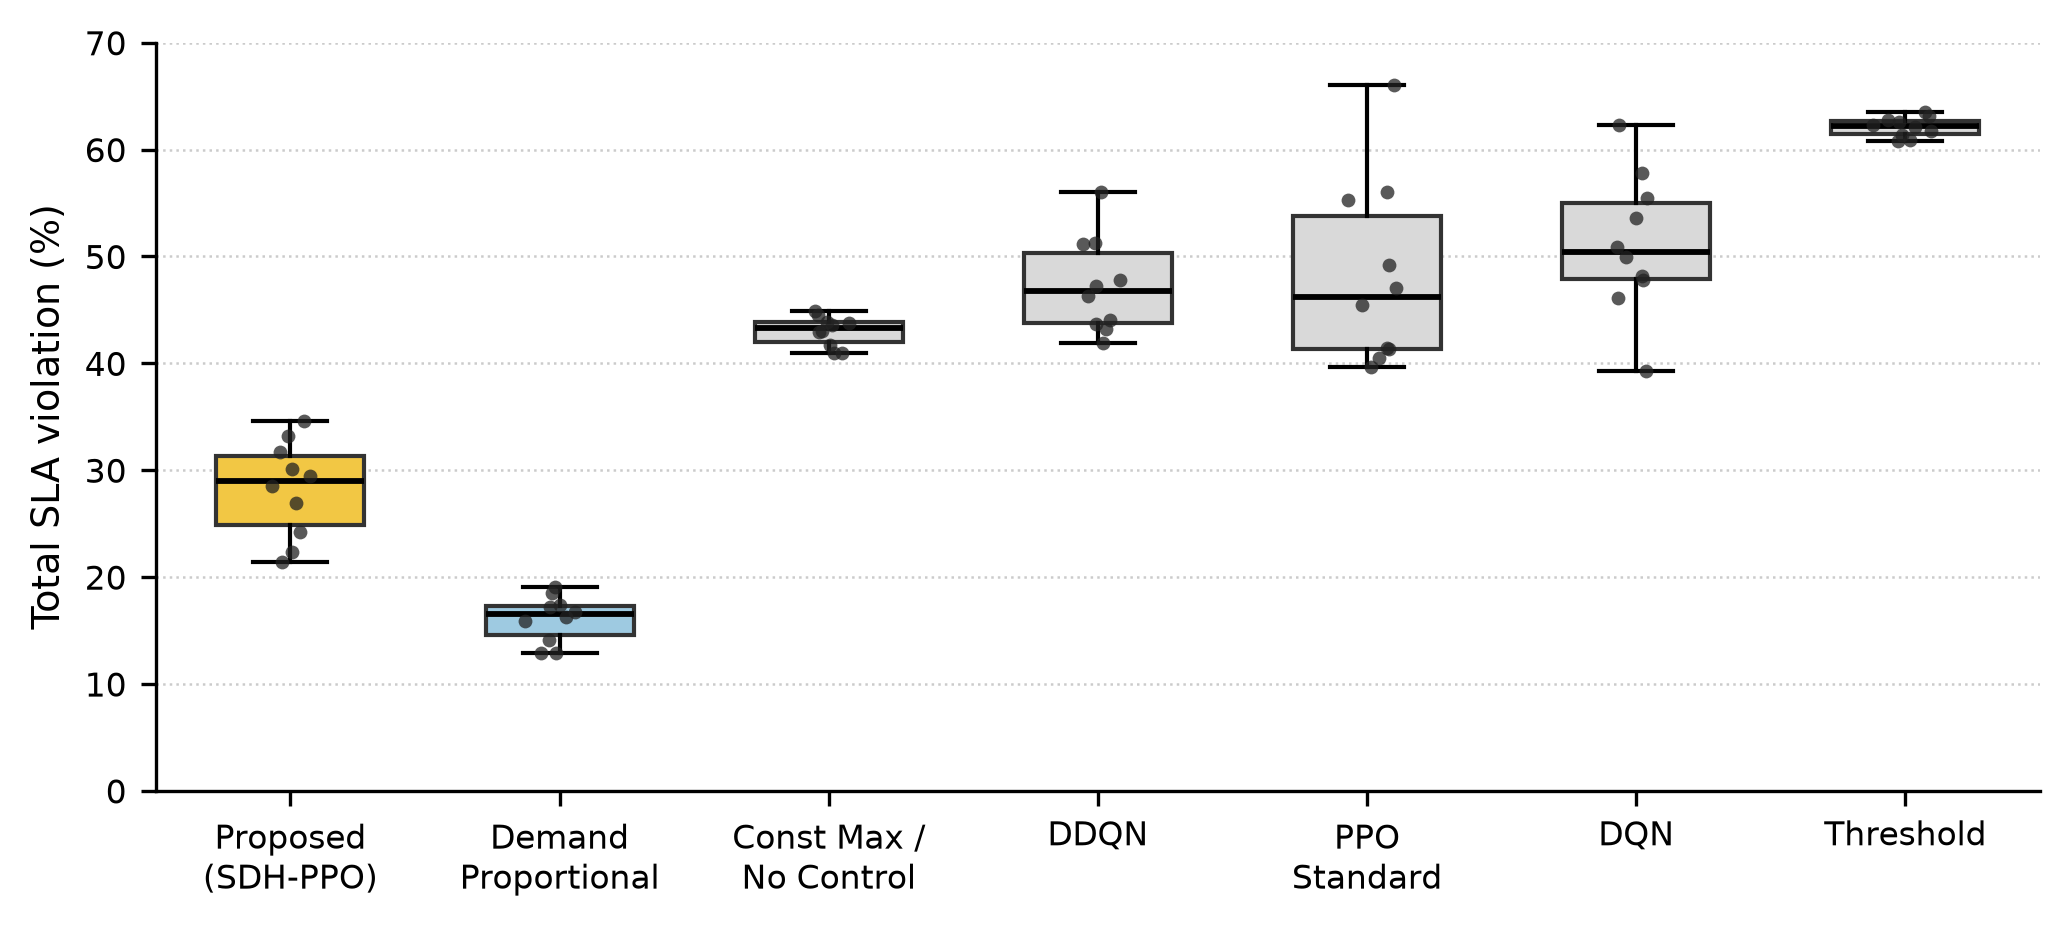
\includegraphics[width=\columnwidth]{figures/fig4_seed_distribution.png}
\caption{\rev{Per-seed total SLA violation rate, 10 seeds per configuration. Each point is one seed.}}
\label{fig:4}
\end{figure}

\begin{table}[htbp]
\centering
\caption{\rev{Significance of Total Violation Rate, Proposed Versus Each Baseline, Holm-Corrected (10 Seeds Each)}}
\label{tab:stats}
\footnotesize
\begin{tabular}{lccl}
\toprule
\revhdr Comparison & $p$ (MWU) & $p$ (Holm) & Verdict \\
\midrule
vs. PPO Standard & 0.0002 & 0.0013 & Proposed better \\
vs. DDQN & 0.0002 & 0.0013 & Proposed better \\
vs. DQN & 0.0002 & 0.0013 & Proposed better \\
vs. Threshold & 0.0002 & 0.0013 & Proposed better \\
vs. Const Max & 0.0002 & 0.0013 & Proposed better \\
vs. No Control & 0.0002 & 0.0013 & Proposed better \\
vs. Demand Proportional & 0.0002 & 0.0013 & \textbf{Proposed worse} \\
\bottomrule
\end{tabular}
\\[3pt]
\parbox{\columnwidth}{\footnotesize \rev{*The rank-biserial effect size is \mbox{$-1.00$} for every row marked better and \mbox{$+1.00$} for the final row, indicating complete separation across seeds in both directions.}}
\end{table}

\rev{Against every learned baseline, SDH-PPO is the stronger policy. It attains a total violation rate of 28.25 percent against 48.19 percent for standard PPO, a relative reduction of 41.4 percent; 51.13 percent for DQN, a reduction of 44.7 percent; and 47.26 percent for DDQN, a reduction of 40.2 percent. All three comparisons reach \mbox{$p = 0.0013$} after Holm correction, with a rank-biserial effect size of \mbox{$-1.00$}, meaning no seed of any baseline reached the violation rate of any seed of the proposed method. The separation is visible directly in Fig.~\mbox{\ref{fig:4}}, where the proposed and baseline distributions do not overlap.}

\rev{The value-based baselines fail in a specific and interpretable way. DQN and DDQN violate the P2 threshold on 99.45 and 99.00 percent of steps respectively, with mean P2 delay near the 200 ms buffer ceiling. Discretizing each slice's rate into 21 bins is too coarse to track the camera slice's bursty arrivals under a contended link, so the backlog on P2 saturates while the agent continues to service the other two slices. This is the granularity limitation identified in Section~\mbox{\ref{sec:rw-value}}, reproduced under controlled conditions.}

\rev{Standard PPO shows the opposite failure: not a systematic bias but an instability. Its confidence interval on P1 delay spans 34.20 to 105.27 ms and on P4 delay 15.87 to 76.23 ms, an order of magnitude wider than the proposed method's. Inspection of the per-seed records shows three of ten seeds collapsing to a degenerate allocation. The safety-margin correction is what removes this failure mode, as the ablation below confirms.}

\rev{The result that most constrains the contribution of this work is the last row of Table~\mbox{\ref{tab:stats}}. Demand Proportional, a rule that divides capacity in proportion to each slice's mean measured demand and involves no learning, achieves 16.10 percent total violation against the proposed method's 28.25 percent. The comparison is significant at the same \mbox{$p = 0.0013$} with an effect size of \mbox{$+1.00$}: the separation is complete in the heuristic's favour. Most of the gap sits on P2, where the proposed method violates on 46.28 percent of steps against the heuristic's 15.08 percent.}

\rev{The explanation is visible in the environment definition. Total mean demand (12.28 Mbps) exceeds link capacity (12 Mbps) by only 2 percent, and the per-slice demands are close to stationary across an episode. Under those conditions a static split proportional to mean demand is very nearly the optimal allocation, and there is little for a policy to exploit by reacting to instantaneous state. A learned controller would be expected to pay off under stronger non-stationarity, correlated bursts, or a tighter capacity margin; none of those conditions holds in the trace collected here. Reporting this is more useful than omitting the baseline, since a reader deploying slice orchestration on a comparably loaded link should prefer the heuristic.}

\subsection{Ablation Study}\label{sec:ablation}

\rev{Table~\mbox{\ref{tab:abl}} isolates the two architectural claims by removing one component at a time and re-running all 10 seeds.}

\begin{table}[htbp]
\centering
\caption{\rev{Ablation of Total Violation Rate, Holm-Corrected (10 Seeds Each)}}
\label{tab:abl}
\footnotesize
\begin{tabular}{lccl}
\toprule
\revhdr Variant & Total Viol (\%) & $p$ (Holm) & Verdict \\
\midrule
Proposed (full) & 28.25 [25.62, 30.88] & --- & --- \\
w/o safety layer & 50.11 [44.17, 56.28] & 0.0004 & Full better \\
w/o Dueling Critic & 27.81 [24.55, 30.13] & 0.9698 & No difference \\
\bottomrule
\end{tabular}
\end{table}

\rev{Removing the safety-margin correction raises total violation from 28.25 to 50.11 percent, a cost of 21.9 percentage points, significant at \mbox{$p = 0.0004$} with an effect size of \mbox{$-1.00$}. The degradation is concentrated on P2, which rises from 46.28 to 94.82 percent, and the confidence interval widens from 5.3 to 12.1 points, reproducing the instability seen in standard PPO. Without the correction, the proposed method performs no better than standard PPO (50.11 against 48.19 percent). The safety layer, not the policy-gradient machinery, accounts for the improvement over PPO reported in Section~\mbox{\ref{sec:comparative}}.}

\rev{Removing the Dueling Critic changes nothing. Total violation moves from 28.25 to 27.81 percent, nominally in favour of the simpler critic, at \mbox{$p = 0.9698$} with an effect size of \mbox{$+0.02$}. This is a null result and is reported as one. The decomposition \mbox{$V(s) + (A(s) - \bar{A})$} is applied to a state-only critic with a single scalar output, so the advantage-residual term cannot discriminate between actions in the way it does in Dueling DQN, where the head spans a discrete action set. The component is retained in the architecture description for completeness, but no performance claim is made for it, and a reimplementation may omit it without loss.}

\subsection{Discussion and Limitations}\label{sec:limitations}

\rev{Four limitations bound the claims above and are stated explicitly rather than left for the reader to infer.}

\rev{\emph{The control results are simulation, not measurement.} The arrival process is replayed from measured traffic, but the mapping from policing rate to delay is derived from queueing theory. The measurement campaign never varied the policing rate, so this mapping was never observed. A sweep over the policing rate on physical hardware, with clock synchronization established beforehand, is the necessary next step; a protocol for it is specified but was not executed for this paper.}

\rev{\emph{Measured delay is not usable as ground truth in its present form.} 13.19 percent of one-way delay samples in the collected trace are negative, which is physically impossible and indicates that the sender and collector clocks were not synchronized. The magnitude of the true queueing signal relative to this offset is unknown. Only the byte-counter-derived throughput columns, which are immune to clock offset, are used here.}

\rev{\emph{The load regime is narrow.} All results are obtained at one capacity setting against one demand profile, at a 2 percent overload. The finding that a demand-proportional heuristic dominates is specific to that regime and should not be generalized without a capacity sweep.}

\rev{\emph{The dueling component is unsupported.} As the ablation shows, it contributes nothing measurable in this configuration, and the paper makes no claim for it.}

\section{Conclusion}\label{sec:conclusion}

\rev{This research presented SDH-PPO, a continuous-action resource orchestration framework for multi-tenant SDN-based IoT environments, and evaluated it against seven baselines in a shared-capacity queueing simulator driven by traces measured on a physical Raspberry Pi testbed, across 10 seeds per configuration with bootstrap confidence intervals and Holm-corrected significance tests.}

\rev{SDH-PPO reduces the total SLA violation rate to 28.25 percent, against 48.19 percent for standard PPO, 51.13 percent for DQN, and 47.26 percent for DDQN. All three comparisons are significant at \mbox{$p = 0.0013$} with complete separation across seeds. An ablation attributes this advantage specifically to the safety-margin correction, whose removal costs 21.9 percentage points (\mbox{$p = 0.0004$}); the Dueling Critic head shows no measurable effect (\mbox{$p = 0.97$}) and no performance claim is made for it. Restating the safety comparison in SLA-relative rather than standardized units is what turns that component from an inert branch into the principal source of the improvement, which suggests that the unit in which a safety constraint is expressed deserves as much attention as the policy that it guards.}

\rev{The framework does not, however, outperform a demand-proportional heuristic, which reaches 16.10 percent under the same protocol with the separation running in the heuristic's favour. At a 2 percent overload against near-stationary per-slice demand, a static proportional split is close to optimal and leaves little for a reactive policy to recover. Establishing where learned orchestration begins to pay off therefore requires a regime with stronger non-stationarity or a tighter capacity margin.}

\rev{Future work follows directly from the limitations of Section~\mbox{\ref{sec:limitations}}: establishing clock synchronization on the testbed and executing a policing-rate sweep, so that the action-to-delay relationship is measured rather than modelled; calibrating the queueing model against that sweep and reporting its prediction error on held-out operating points; and repeating the comparison across a range of capacity margins to identify the load regime in which a learned policy overtakes the proportional heuristic.}

\begin{thebibliography}{50}
\bibitem{b1} S. Wijethilaka and M. Liyanage, ``Survey on Network Slicing for Internet of Things Realization in 5G Networks,'' Apr. 01, 2021, \emph{Institute of Electrical and Electronics Engineers Inc.} doi: 10.1109/COMST.2021.3067807.

\bibitem{b2} V. Sharma, ``Performance Evaluation of Network Slicing in 5G Core Networks,'' \emph{International Journal of Multidisciplinary Research and Growth Evaluation}, vol. 3, no. 5, pp. 648--654, 2022, doi: 10.54660/.ijmrge.2022.3.5.648-654.

\bibitem{b3} E. Thomatos, A. Sgora, A. Tsipis, and P. Chatzimisios, ``AI Methods in Network Slice Life-Cycle Phases: A Survey,'' Oct. 01, 2025, \emph{Multidisciplinary Digital Publishing Institute (MDPI)}. doi: 10.3390/electronics14204053.

\bibitem{b4} W. He, H. Yao, H. Chang, and Y. Liu, ``A P4-Based Approach to Traffic Isolation and Bandwidth Management for 5G Network Slicing,'' \emph{Tsinghua Sci. Technol.}, vol. 30, no. 1, pp. 171--185, Sep. 2024, doi: 10.26599/tst.2024.9010020.

\bibitem{b5} Y. Safaei, P. Arefijamal, M. Siamaki, and B. Safaei, ``Priority-Aware SDN Orchestration for Surgical IoMT: A Joint Optimization of Hit Ratio and Latency With Dynamic Resource Reallocation,'' \emph{IEEE Access}, vol. 13, pp. 113787--113808, 2025, doi: 10.1109/ACCESS.2025.3583899.

\bibitem{b6} V. Onaji, E. Adediji, J. Njimgou, K. Ayano, and D. Olufemi, ``Deep Reinforcement Learning for Dynamic Network Slicing and Resource Orchestration in Software-Defined Critical Telecom Infrastructure,'' \emph{International Journal of Computer Applications Technology and Research}, Nov. 2025, doi: 10.7753/ijcatr1411.1006.

\bibitem{b7} P. Jangale, ``Impact of Network Slicing on Performance in 5G and Beyond,'' \emph{Journal of Artificial Intelligence, Machine Learning and Data Science}, vol. 1, no. 1, pp. 1653--1657, Nov. 2022, doi: 10.51219/jaimld/pratik-jangale/368.

\bibitem{b8} S. T. Arzo \emph{et al.}, ``MSN: A Playground Framework for Design and Evaluation of MicroServices-Based SDN Controller,'' \emph{Journal of Network and Systems Management}, vol. 30, no. 1, Jan. 2022, doi: 10.1007/s10922-021-09631-7.

\bibitem{b9} R. Pérez, M. Rivera, Y. Salgueiro, C. R. Baier, and P. Wheeler, ``Moving Microgrid Hierarchical Control to an SDN-Based Kubernetes Cluster: A Framework for Reliable and Flexible Energy Distribution,'' \emph{Sensors}, vol. 23, no. 7, Apr. 2023, doi: 10.3390/s23073395.

\bibitem{b10} V. Kumar Sharma, ``Cloud-Native 5G Deployments: Kubernetes and Microservices in Telco Networks,'' \emph{International Journal of Innovative Research in Engineering \& Multidisciplinary Physical Sciences}, vol. 10, no. 3, pp. 1--8, 2022, {[}Online{]}. Available: www.ijirmps.org

\bibitem{b11} A. Kamisetty, D. Narsina, M. Rodriguez, S. Kothapalli, J. Chandra, and S. Gummadi, ``Microservices vs. Monoliths: Comparative Analysis for Scalable Software Architecture Design,'' \emph{Engineering International}, vol. 11, no. 2, 2023.

\bibitem{b12} S. T. Arzo, D. Scotece, R. Bassoli, M. Devetsikiotis, L. Foschini, and F. H. P. Fitzek, ``Softwarized and containerized microservices-based network management analysis with MSN,'' \emph{Computer Networks}, vol. 254, Dec. 2024, doi: 10.1016/j.comnet.2024.110750.

\bibitem{b13} Y. Xu and Q. Yu, ``Deep reinforcement learning based computation offloading and resource allocation strategy for maritime internet of things,'' \emph{Computer Networks}, vol. 264, Jun. 2025, doi: 10.1016/j.comnet.2025.111221.

\bibitem{b14} B. M. Alrifai, L. Alsbatin, and F. Zawaideh, ``Optimizing 5G Resource Allocation with Reinforcement Learning: A Q-Learning and Deep Q-Network (DQN) Approach,'' \emph{Journal of Advances in Information Technology}, vol. 16, no. 11, pp. 1586--1594, 2025, doi: 10.12720/jait.16.11.1586-1594.

\bibitem{b15} M. Hosseinzadeh \emph{et al.}, ``SDN-Based NFV deployment for multi-objective resource allocation in edge computing: A deep reinforcement learning for iot workload scheduling,'' \emph{Sustainable Computing: Informatics and Systems}, vol. 48, Dec. 2025, doi: 10.1016/j.suscom.2025.101218.

\bibitem{b16} V. Sittakul, I. Ioannou, P. Nagaradjane, and V. Vassiliou, ``Intelligent congestion control in 5G URLLC Software-Defined Networks using adaptive resource management via Reinforced Dueling Deep Q-Networks,'' \emph{Journal of Network and Computer Applications}, vol. 242, Oct. 2025, doi: 10.1016/j.jnca.2025.104276.

\bibitem{b17} A. Iqbal, A. Nauman, T. Khurshaid, and S. B. Rhee, ``A Scalable Reinforcement Learning Framework for Ultra-Reliable Low-Latency Spectrum Management in Healthcare Internet of Things,'' \emph{Mathematics}, vol. 13, no. 18, Sep. 2025, doi: 10.3390/math13182941.

\bibitem{b18} M. Chahoud \emph{et al.}, ``Reward shaping in DRL: A novel framework for adaptive resource management in dynamic environments,'' \emph{Inf. Sci. (N. Y).}, vol. 715, Oct. 2025, doi: 10.1016/j.ins.2025.122238.

\bibitem{b19} A. Abderrahmane, H. Drid, and A. Behaz, ``A Survey of Controller Placement Problem in SDN-IoT Network,'' Dec. 01, 2024, \emph{Springer Science and Business Media B.V.} doi: 10.1007/s44227-024-00035-y.

\bibitem{b20} R. Botez, J. Costa-Requena, I. A. Ivanciu, V. Strautiu, and V. Dobrota, ``SDN-based network slicing mechanism for a scalable 4G/5G core network: A Kubernetes approach,'' \emph{Sensors}, vol. 21, no. 11, Jun. 2021, doi: 10.3390/s21113773.

\bibitem{b21} J. M. Fernandez, I. Vidal, and F. Valera, ``Enabling the orchestration of IoT slices through edge and cloud microservice platforms,'' \emph{Sensors (Switzerland)}, vol. 19, no. 13, Jul. 2019, doi: 10.3390/s19132980.

\bibitem{b22} Y. Zhang, C. Li, N. Chen, and P. Zhang, ``Intelligent Requests Orchestration for Microservice Management Based on Blockchain in Software Defined Networking: A Security Guarantee,'' in \emph{2022 IEEE International Conference on Communications Workshops, ICC Workshops 2022}, Institute of Electrical and Electronics Engineers Inc., 2022, pp. 254--259. doi: 10.1109/ICCWorkshops53468.2022.9814536.

\bibitem{b23} F. Tonini, C. Natalino, M. Furdek, C. Raffaelli, and P. Monti, ``Network Slicing Automation: Challenges and Benefits,'' in \emph{2020 24th International Conference on Optical Network Design and Modeling, ONDM 2020}, 2020. doi: 10.23919/ONDM48393.2020.9133004.

\bibitem{b24} S. Sriharsha Rachakonda and R. Lakshmikanth, ``Enhancing Network Security With QoS-Aware Optimization Models In 6G Network Slicing Architectures.'' {[}Online{]}. Available: https://www.theaspd.com/ijes.php

\bibitem{b25} P. Kochovski, U. Paščinski, V. Stankovski, and M. Ciglarič, ``Pareto-Optimised Fog Storage Services with Novel Service-Level Agreement Specification,'' \emph{Applied Sciences (Switzerland)}, vol. 12, no. 7, Apr. 2022, doi: 10.3390/app12073308.

\bibitem{b26} K. Zia, A. Chiumento, P. Havinga, R. Riggio, and Y. Huang, ``QoS Aware Slice Resource Management Using Deep Reinforcement Learning in IoT Networks,'' in \emph{2023 19th International Conference on Distributed Computing in Smart Systems and the Internet of Things (DCOSS-IoT)}, Jan. 2023, pp. 150--154. doi: 10.1109/DCOSS-IoT58021.2023.00035.

\bibitem{b27} F. Mason, G. Nencioni, and A. Zanella, ``Using Distributed Reinforcement Learning for Resource Orchestration in a Network Slicing Scenario,'' \emph{IEEE/ACM Transactions on Networking}, vol. 31, no. 1, pp. 88--102, 2023, doi: 10.1109/TNET.2022.3187310.

\bibitem{b28} S. Venkatapathy, T. Srinivasan, O. S. Lee, R. Jayaraman, H. G. Jo, and I. H. Ra, ``Slice-aware 5G network orchestration framework based on dual-slice isolation and management strategy (D-SIMS),'' \emph{Sci. Rep.}, vol. 14, no. 1, Dec. 2024, doi: 10.1038/s41598-024-68892-9.

\bibitem{b29} H. She, L. Yan, X. An, C. Mao, and Y. Guo, ``Flow persona: A QoS Flow Rule Scheme based on Deep Learning in SDN-IoT,'' \emph{Computer Networks}, vol. 273, 2025, doi: 10.1016/j.comnet.2025.111784.

\bibitem{b30} A. Holscher, M. Asplund, and F. Boeira, ``Evaluation of an SDN-based Microservice Architecture,'' in \emph{Proceedings of the 2022 IEEE International Conference on Network Softwarization, NetSoft 2022}, 2022, pp. 151--156. doi: 10.1109/NetSoft54395.2022.9844094.

\bibitem{b31} M. Zambianco and G. Verticale, ``Intelligent multi-branch allocation of spectrum slices for inter-numerology interference minimization,'' \emph{Computer Networks}, vol. 196, 2021, doi: 10.1016/j.comnet.2021.108254.

\bibitem{b32} M. F. Ul Islam, S. Hossain, M. G. R. Alam, N. Mansoor, and A. Chakrabarty, ``Optimizing network bandwidth slicing identification: NADAM-enhanced CNN and VAE data preprocessing for enhanced interpretability,'' \emph{PLoS One}, vol. 20, no. 10, Oct. 2025, doi: 10.1371/journal.pone.0333286.

\bibitem{b33} L. Zhao, Y. Liu, A. Hawbani, N. Lin, W. Zhao, and K. Yu, ``QoS-Aware Multihop Task Offloading in Satellite--Terrestrial Edge Networks,'' \emph{IEEE Internet Things J.}, vol. 11, no. 19, pp. 31453--31466, Oct. 2024, doi: 10.1109/JIOT.2024.3417456.

\bibitem{b34} C. Ssengonzi, O. P. Kogeda, and T. O. Olwal, ``A survey of deep reinforcement learning application in 5G and beyond network slicing and virtualization,'' \emph{Array}, vol. 14, 2022, doi: 10.1016/j.array.2022.100142.

\bibitem{b35} T. Mai, H. Yao, N. Zhang, W. He, D. Guo, and M. Guizani, ``Transfer Reinforcement Learning Aided Distributed Network Slicing Optimization in Industrial IoT,'' \emph{IEEE Transactions on Industrial Informatics}, vol. 18, no. 6, pp. 4308--4316, Jun. 2022, doi: 10.1109/TII.2021.3132136.

\bibitem{b36} D. H. Abdulazeez and S. K. Askar, ``Offloading Mechanisms Based on Reinforcement Learning and Deep Learning Algorithms in the Fog Computing Environment,'' \emph{IEEE Access}, vol. 11, pp. 12554--12585, 2023, doi: 10.1109/ACCESS.2023.3241881.

\bibitem{b37} C. Tan, ``Comparative Study of Reinforcement Learning Performance Based on PPO and DQN Algorithms,'' \emph{Applied and Computational Engineering}, vol. 175, pp. 30--36, 2025.

\bibitem{b38} M. Arjovsky, S. Chintala, and L. Bottou, ``Wasserstein Generative Adversarial Networks,'' in \emph{Proceedings of the 34th International Conference on Machine Learning (ICML)}, PMLR, 2017, pp. 214--223.

\bibitem{b39} I. Gulrajani, F. Ahmed, M. Arjovsky, V. Dumoulin, and A. Courville, ``Improved Training of Wasserstein GANs,'' in \emph{Advances in Neural Information Processing Systems (NeurIPS)}, vol. 30, 2017.

\bibitem{b40} Q. Liu, N. Choi, and T. Han, ``OnSlicing: Online End-to-End Network Slicing with Reinforcement Learning,'' in \emph{Proceedings of the 17th International Conference on emerging Networking EXperiments and Technologies (CoNEXT)}, 2021, doi: 10.1145/3485983.3494850.

\bibitem{b41} A. M. Nagib, H. Abou-Zeid, and H. S. Hassanein, ``SafeSlice: Enabling SLA-Compliant O-RAN Slicing via Safe Deep Reinforcement Learning,'' in \emph{2025 IEEE International Conference on Machine Learning for Communication and Networking (ICMLCN)}, 2025.

\bibitem{b42} Q. Qi \emph{et al.}, ``Augmented Lagrangian-Based Reinforcement Learning for Network Slicing in IIoT,'' \emph{Electronics}, vol. 11, no. 20, p. 3385, 2022, doi: 10.3390/electronics11203385.

\bibitem{b43} W. Wang, M. Li, and H. Wu, ``HyAR-PPO: Hybrid Action Representation Learning for Incentive-Driven Task Offloading in Vehicular Edge Computing,'' \emph{Sensors}, vol. 26, no. 6, p. 1743, 2026, doi: 10.3390/s26061743.

\bibitem{b44} A. Alchaab, A. Younis, and D. Pompili, ``Slice-on-the-Fly: AI-based Network Slicing in O-RAN for Dynamic Traffic Demands,'' in \emph{2025 IEEE 26th International Symposium on a World of Wireless, Mobile and Multimedia Networks (WoWMoM)}, 2025, pp. 51--60.

\bibitem{b45} ``Slice-Aware and Computationally Efficient Resource Orchestration for Converged mmWave-PON O-RAN: A Reward-Shaped PPO Approach for Joint DBA and PRB Allocation,'' \emph{Telecom}, vol. 7, no. 3, p. 75, 2026.

\bibitem{b46} L. Tarkh, A. Chouman, H. Lutfiyya, and A. Shami, ``RL-Loop: Reinforcement Learning-Driven Real-Time 5G Slice Control for Connected and Autonomous Mobility Services,'' \emph{arXiv preprint arXiv:2604.02461}, 2026.

\bibitem{b47} X. Bai, M. T. Islam, R. Buyya, and A. N. Toosi, ``REACH: Reinforcement Learning for Adaptive Microservice Rescheduling in the Cloud-Edge Continuum,'' \emph{arXiv preprint arXiv:2510.06675}, 2025.

\bibitem{b48} C. Song, M. Xu, K. Ye, H. Wu, S. S. Gill, R. Buyya, and C. Xu, ``ChainsFormer: A Chain Latency-Aware Resource Provisioning Approach for Microservices Cluster,'' in \emph{International Conference on Service-Oriented Computing (ICSOC)}, 2023, doi: 10.1007/978-3-031-48421-6\_14.

\bibitem{b49} Y. Liu, J. Ding, and X. Liu, ``Resource Allocation Method for Network Slicing Using Constrained Reinforcement Learning,'' in \emph{IEEE International Conference on Network Protocols (ICNP)}, 2020.

\bibitem{b50} R. Raftopoulos, S. D'Oro, \emph{et al.}, ``DRL-based Latency-Aware Network Slicing in O-RAN with Time-Varying SLAs,'' in \emph{International Conference on Computing, Networking and Communications (ICNC)}, 2024.

\end{thebibliography}

\end{document}
